% Changed: restructure for a single evidence-bound service-object argument.
% Protected: measured values, protocol distinctions and failure records.
% Meaning-Check: PRESERVED
% Risk-Flags: none
\section{Introduction}
\label{sec:introduction}

Consider a retrieval service that sends the current question before a long set of source documents. Two authorized users ask different questions about the same documents. Almost all of the document text repeats, yet native prefix caching stops at the first changed question token. This order occurs in a fixed revision of Azure's public RAG demonstration, whose conversation history and question precede the retrieved sources~\cite{azuretemplate}. The opportunity is concrete: move reusable context ahead of changing fields, and subsequent requests can reuse a longer physical KV prefix.

The difficulty is deciding when that transformed state is suitable for a shared service. A dependency-valid reorder can still change an autoregressive model's answer. A development NarrativeQA case retained its compiled witness when metadata changed the raw answer (Section~\ref{sec:quality}). A speculative candidate can also enter the shared cache before its qualification finishes. These are linked service decisions: admissible layout, applicable behavioral evidence, and authorized publication. Addressing only the layout leaves later tenants dependent on an unchecked execution artifact.

Existing systems establish several ways to exploit repeated context. PagedAttention and RadixAttention manage exact-prefix sharing~\cite{vllm2023,sglang2024}; Prompt Cache exposes reusable modules~\cite{promptcache2024}; CacheBlend and EPIC reuse context across positions through different execution mechanisms~\cite{cacheblend2025,epic2025}. Application-aware systems such as Parrot expose dependencies to the serving layer~\cite{parrot2024}; row/field reordering also improves reuse in relational analytics~\cite{llmqueries2025}. ContractKV addresses the complementary control-plane question: \emph{what evidence and identity permit a transformed prefix to become shared state?}

We argue that reusable KV should be governed as a service object: its layout, behavioral evidence and transactional visibility must share one validity binding. The same binding that authorizes a compiled layout governs the state visible to later requests. Four mechanisms implement this idea. The \emph{Contract-Aware Layout Compiler} (CALC) exposes stable leading content while preserving registered dependencies. \emph{Scoped Behavioral Certification} associates model-backed token-path evidence with an input and execution scope. \emph{Prefix-Selective Transactional Promotion} (PSTP) keeps candidate state private until a valid pass, then commits only the eligible stable blocks. A \emph{Service-Template Certificate} binds identity, authorization, and lifecycle so that qualified requests can share the object and its admission cost.

\begin{figure*}[t]
\centering
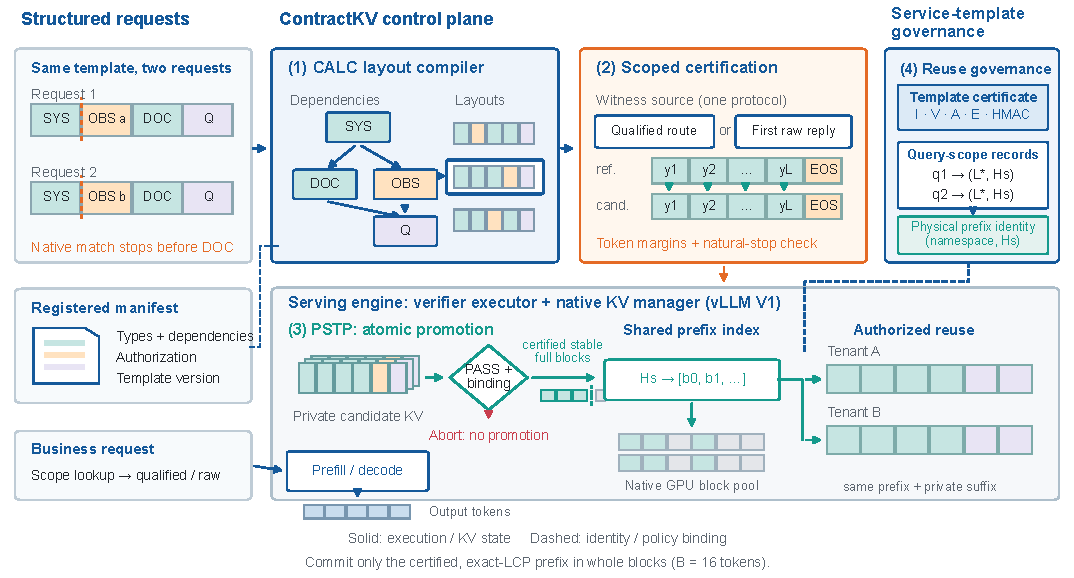
\includegraphics[width=\textwidth]{figures/fig1_architecture.pdf}
\caption{ContractKV makes a compiled stable prefix an evidence-bound service object. CALC repairs a structural prefix gap; one of two separately evaluated witness protocols supplies scoped token-path evidence; PSTP commits eligible state only after PASS and a valid binding. Authorized tenants of the same template share the prefix and keep changing suffixes private. The deployment certificate and controlled-client query records are distinct (Table~\ref{tab:qualification-protocols}); their prefix associations refer to the same physical object. The commit cut excludes incomplete blocks and private suffixes.}
\label{fig:architecture}
\end{figure*}

The Service-Template Certificate makes the prefix and its qualification cost shareable under versioned authorization. Distinct behavioral scopes may refer to the same physical object. Section~\ref{sec:scope} defines the witness and cost units for deployment-qualified registration and stricter query-qualified execution.

The evaluation closes the argument from two directions. First, six source-disjoint HotpotQA/RepoBench templates yield 1.619$\times$, 1.109$\times$, and 1.070$\times$ zero-slack full-cost throughput across three models; all 1,296 admitted compiled future pairs preserve raw output IDs. Second, deployment controls hold layout fixed while template scope reduces verifier calls 25-fold and unhidden verification exposure 7.7-fold. A separate open-arrival study adds 0.658 compliant requests/s at its fixed 80\%-load point, and density replay over 10--80 authorized identities demonstrates physical consolidation. These results test behavioral admissibility and service economics within their respective protocols.

The paper makes four contributions, each connecting a mechanism to observable service behavior:
\begin{itemize}
\item \textbf{Contract-aware compilation} of bounded, dependency-valid layout candidates with exact rendered-token identities (Section~\ref{sec:calc}).
\item \textbf{Scoped model-backed admission} that binds token-path and termination evidence to declared inputs and execution conditions, evaluated with real free-running generation (Sections~\ref{sec:scope} and~\ref{sec:quality}).
\item \textbf{Transactional KV publication} at an exact-LCP, block-aligned commit boundary, with zero promotion for rejected candidates (Sections~\ref{sec:pstp} and~\ref{sec:ablation}).
\item \textbf{Service-Template Certificates} that bind authorized, versioned prefix reuse to its lifecycle and make qualification shareable across tenants, with measured 25-fold call amortization, SLO service benefit and physical consolidation (Sections~\ref{sec:template}, \ref{sec:mainresults}, and~\ref{sec:deployment}).
\end{itemize}
